\documentclass[dvipdfmx,12pt,aspectratio=169]{beamer}
%aspectratioは横縦比16:9，1610とすれば16:10に．省けば4:3に．
%ノートPCの画面サイズを調べて，合わせましょう．
%フォントサイズは11pt,12ptなどもありますが，12ptか14ptが良いでしょう
\usepackage{graphicx}
\usepackage{xcolor} %tcolorboxで色を変えたから
\usepackage{bxdpx-beamer}% dvipdfmxなので必要
\usepackage{pxjahyper}% 日本語で'しおり'したい
\usepackage{minijs}% min10ヤダ
\renewcommand{\kanjifamilydefault}{\gtdefault}% 既定をゴシック体に

\usetheme{Boadilla}
%themeは https://tex.y-misc.org/beamer/theme.html を参照
\setbeamercovered{transparent}%消えている文字をうっすらと表示する
\usepackage{tcolorbox} %色を変えたboxを使うなら．
\usepackage{hyperref}

\usepackage{amsmath} %align環境などの数式環境に
\usepackage{amssymb} %特殊な数式シンボルに必須
\usepackage{amsthm} %theorem環境に．
%上の３つは{amsmath,amssymb,amsthm}とまとめても．
\renewcommand\proofname{\bf 証明} %Proofではなく証明


\usepackage{tikz}%お絵描きするなら必要



\theoremstyle{definition} %見出しは太字，本文で斜体を使わない
\newtheorem{dfn}{定義}
\newtheorem{thm}[dfn]{定理}
\newtheorem{prp}[dfn]{命題}
\newtheorem{lmm}[dfn]{補題}


\definecolor{forestgreen}{rgb}{0.13, 0.55, 0.13}
%forestgreen色を使いたかった

%%%%%%%%%%%%%%%%%%%%%%%%%%%%%%%%%%%%%%%%%%%%%%%%%%%%%%%%%%%%%
%%%%%%%%%%%%%%%%%%%%%%%プリアンブル終り%%%%%%%%%%%%%%%%%%%%%%
%%%%%%%%%%%%%%%%%%%%%%%%%%%%%%%%%%%%%%%%%%%%%%%%%%%%%%%%%%%%%
\title{.goで作る最良近似多項式}
\author{imohiyoko}
\date{2025年11月16日(土)}
\titlegraphic{%
 \begin{tikzpicture}[remember picture, overlay]
  \node[anchor=south east, % ノードの「南東（右下）」を基準にする
        xshift=-2cm,      % ページの右端から1cm左へ
        yshift=2cm]       % ページの下端から1cm上へ
        at (current page.south east) % ページの「南東（右下）」を基準位置に
  {
\includegraphics[width=3cm]{./material/go-img.png}}; % 挿入する画像
 \end{tikzpicture}%
}
\begin{document}
\maketitle
\begin{frame}{目次}
 \begin{itemize}
  \item 最良近似多項式とは？
  \item go言語ってなに?(趣味の話)
  \item どんな構成?
  \item 実際に動かしてみる
 \end{itemize}
\end{frame}

\section{最良近似多項式とは？}
\begin{frame}{最良近似多項式とは}
 \begin{dfn}
 与えられた連続関数 $f(x)$ を多項式 $P(x)$ で近似する問題を考え，近似の度合いは誤差の一様ノルム
 \[ ||f-P||_{\infty} = \max_{x\in[a,b]} |f(x)-P(x)| \]
 で測るものとする．このとき，$P(x)$ の次数を $n$ 次以下 ($\mathcal{P}_n$) に限る場合に，近似誤差の下限
 \[ E_n(f) = \inf_{P\in\mathcal{P}_n} ||f-P||_{\infty} \]
 を与える $P=P^* \in \mathcal{P}_n$ を $f$ の $n$ 次最良近似多項式と呼ぶ．
 \end{dfn}
\end{frame}
\begin{frame}
  \begin{block}{最良誤差関数の特徴}
    \begin{itemize}
      \item 最良近似多項式はどのような関数にたいしても存在する．
      \item 最良近似多項式は一意に存在する．
      \item 最良近似多項式の誤差関数 $f(x)-P^*(x)$ は，少なくとも $n+2$ 個の交互に変わる極値点を持つ．
    \end{itemize}
  \end{block}
\end{frame}

\begin{frame}{最良誤差関数の特徴}
  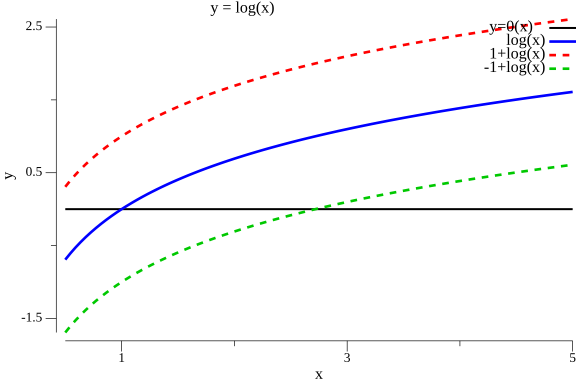
\includegraphics[width=0.8\linewidth]{./material/log-tohaba.png}
\end{frame}

\section{GO言語ってなに?(趣味の話)}
\begin{frame}
  \frametitle{なぜGoなのか}
  \framesubtitle{Googleが直面していた「開発の壁」}
  
  \begin{itemize}
    \item \textbf{C++の複雑性}
    \begin{itemize}
        \item 高機能だが複雑すぎる．コードの可読性・保守性が低下．
    \end{itemize}
    
    \item \textbf{遅いコンパイル時間}
    \begin{itemize}
        \item 大規模プロジェクトではビルドに数時間．生産性が著しく低下．
    \end{itemize}
    
    \item \textbf{マルチコアの活用}
    \begin{itemize}
        \item 既存言語での安全な「並行処理」は非常に困難だった．
    \end{itemize}
  \end{itemize}
  
  \begin{alertblock}{Goの設計目標}
    C/C++の「実行速度」 + Pythonの「書きやすさ」 + 「高速コンパイル」
  \end{alertblock}
\end{frame}

\begin{frame}
  \frametitle{Go / C / C++ / Python 比較表}
  \begin{tabular}{|l|l|l|l|l|} \hline
  比較項目 & Go & C & C++ & Python \\ \hline
  実行速度 & 速い & 超高速 & 超高速 & 低速 \\
  コンパイル速度 & \alert{超速} & 速い & \alert{遅い} & 不要 \\
  処理の並列化 & \alert{簡単} & 難しい & 難しい & \alert{苦手 (GILの制約)} \\
  メモリ管理 & 自動 & 手動 & 手動 & 自動 \\ 
  型定義 & 静的 & 静的 & 静的 & 動的 \\
  主な用途 & \alert{大規模システム} & システム & \alert{システム, ゲーム} & \alert{Web, AI} \\ \hline
  \end{tabular}
\end{frame}

\section{どんな構成?}
\begin{frame}
\href{run:./material/README.png}{関数一覧}

\href{run:./material/remesAlgorithm.png}{ワークフロー図}

\end{frame}

\section{実際に動かしてみる}

\begin{frame}{最大誤差の収束}
  \centering % 画像を中央に配置
  \includegraphics[width=0.8\linewidth]{./../go-plot/iteration-max-error.png} % ← ここにファイルパスを指定
  \vspace{0.5cm} % 画像の下に少しスペースを開ける
  このグラフは，データ分析の結果を示しています．
\end{frame}

\begin{frame}{最良近似-イテレーション01}
  \centering % 画像を中央に配置
  \includegraphics[width=0.8\linewidth]{./../go-plot/iter01-func.png} % ← ここにファイルパスを指定
  \vspace{0.5cm} % 画像の下に少しスペースを開ける
  このグラフは，データ分析の結果を示しています．
\end{frame}
\begin{frame}{最良近似-イテレーション02}
  \centering % 画像を中央に配置
  \includegraphics[width=0.8\linewidth]{./../go-plot/iter02-func.png} % ← ここにファイルパスを指定
  \vspace{0.5cm} % 画像の下に少しスペースを開ける
  このグラフは，データ分析の結果を示しています．
\end{frame}
\begin{frame}{最良近似-イテレーション03}
  \centering % 画像を中央に配置
  \includegraphics[width=0.8\linewidth]{./../go-plot/iter03-func.png} % ← ここにファイルパスを指定
  \vspace{0.5cm} % 画像の下に少しスペースを開ける
  このグラフは，データ分析の結果を示しています．
\end{frame}
\begin{frame}{最良近似-イテレーション04}
  \centering % 画像を中央に配置
  \includegraphics[width=0.8\linewidth]{./../go-plot/iter04-func.png} % ← ここにファイルパスを指定
  \vspace{0.5cm} % 画像の下に少しスペースを開ける
  このグラフは，データ分析の結果を示しています．
\end{frame}
\begin{frame}{最良近似-イテレーション05}
  \centering % 画像を中央に配置
  \includegraphics[width=0.8\linewidth]{./../go-plot/iter05-func.png} % ← ここにファイルパスを指定
  \vspace{0.5cm} % 画像の下に少しスペースを開ける
  このグラフは，データ分析の結果を示しています．
\end{frame}
\begin{frame}{最良近似-イテレーション06}
  \centering % 画像を中央に配置
  \includegraphics[width=0.8\linewidth]{./../go-plot/iter06-func.png} % ← ここにファイルパスを指定
  \vspace{0.5cm} % 画像の下に少しスペースを開ける
  このグラフは，データ分析の結果を示しています．
\end{frame}
\begin{frame}{最良近似-イテレーション07}
  \centering % 画像を中央に配置
  \includegraphics[width=0.8\linewidth]{./../go-plot/iter07-func.png} % ← ここにファイルパスを指定
  \vspace{0.5cm} % 画像の下に少しスペースを開ける
  このグラフは，データ分析の結果を示しています．
\end{frame}
\begin{frame}{最良近似-イテレーション08}
  \centering % 画像を中央に配置
  \includegraphics[width=0.8\linewidth]{./../go-plot/iter08-func.png} % ← ここにファイルパスを指定
  \vspace{0.5cm} % 画像の下に少しスペースを開ける
  このグラフは，データ分析の結果を示しています．
\end{frame}

\begin{frame}{誤差関数-イテレーション01}
  \centering % 画像を中央に配置
  \includegraphics[width=0.8\linewidth]{./../go-plot/iter01-error.png} % ← ここにファイルパスを指定
  % \includegraphics[height=0.6\textheight]{your_graph.png} など，高さで指定も可能
  \vspace{0.5cm} % 画像の下に少しスペースを開ける
  このグラフは，データ分析の結果を示しています．
\end{frame}
\begin{frame}{誤差関数-イテレーション02}
  \centering % 画像を中央に配置
  \includegraphics[width=0.8\linewidth]{./../go-plot/iter02-error.png} % ← ここにファイルパスを指定
  \vspace{0.5cm} % 画像の下に少しスペースを開ける
  このグラフは，データ分析の結果を示しています．
\end{frame}
\begin{frame}{誤差関数-イテレーション03}
  \centering % 画像を中央に配置
  \includegraphics[width=0.8\linewidth]{./../go-plot/iter03-error.png} % ← ここにファイルパスを指定
  \vspace{0.5cm} % 画像の下に少しスペースを開ける
  このグラフは，データ分析の結果を示しています．
\end{frame}
\begin{frame}{誤差関数-イテレーション04}
  \centering % 画像を中央に配置
  \includegraphics[width=0.8\linewidth]{./../go-plot/iter04-error.png} % ← ここにファイルパスを指定
  \vspace{0.5cm} % 画像の下に少しスペースを開ける
  このグラフは，データ分析の結果を示しています．
\end{frame}
\begin{frame}{誤差関数-イテレーション05}
  \centering % 画像を中央に配置
  \includegraphics[width=0.8\linewidth]{./../go-plot/iter05-error.png} % ← ここにファイルパスを指定
  \vspace{0.5cm} % 画像の下に少しスペースを開ける
  このグラフは，データ分析の結果を示しています．
\end{frame}
\begin{frame}{誤差関数-イテレーション06}
  \centering % 画像を中央に配置
  \includegraphics[width=0.8\linewidth]{./../go-plot/iter06-error.png} % ← ここにファイルパスを指定
  \vspace{0.5cm} % 画像の下に少しスペースを開ける
  このグラフは，データ分析の結果を示しています．
\end{frame}
\begin{frame}{誤差関数-イテレーション07}
  \centering % 画像を中央に配置
  \includegraphics[width=0.8\linewidth]{./../go-plot/iter07-error.png} % ← ここにファイルパスを指定
  \vspace{0.5cm} % 画像の下に少しスペースを開ける
  このグラフは，データ分析の結果を示しています．
\end{frame}
\begin{frame}{誤差関数-イテレーション08}
  \centering % 画像を中央に配置
  \includegraphics[width=0.8\linewidth]{./../go-plot/iter08-error.png} % ← ここにファイルパスを指定
  \vspace{0.5cm} % 画像の下に少しスペースを開ける
  このグラフは，データ分析の結果を示しています．
\end{frame}
\end{document}
